% CHEAT SHEET for the Reliable and Interpretable Artificial Intelligence Lecture
% Autumn 2018 ETH Zurich (ETHZ)
%
% By Manuel Breitenstein, github.com/manuelbre
%
% Based on the Lecture Slides to be found here: https://www.sri.inf.ethz.ch/teaching/riai2018
%
% Latex Template based on the MACHINE LEARNING HS 2017 Cheat Sheet by JONAS EICHENBERGER
% 
% -------------------------------------------------------------


\documentclass[11pt]{extarticle}

\usepackage[
	a4paper,
	landscape,
	left=0.1cm,
	right=0.1cm,
	top=0.1cm,
	bottom=0.1cm,
	includehead,
]{geometry}

\renewcommand{\familydefault}{\sfdefault} % set font 
\newcommand\tab[1][0.25cm]{\hspace*{#1}}

%no page numbers
\pagenumbering{gobble}

% Nice headers
\usepackage{fancyhdr}
% titlepage 
\fancypagestyle{titlepage}{
	\fancyhf{}
	\rhead{\textit{Y.N \& T.E} -- \today}
	\lhead{\textbf{Machine Learning - HS 2017}}
	\cfoot{}
	\setlength{\headheight}{6pt}
	\setlength{\headsep}{8pt}
	\setlength{\footskip}{0pt}
	\setlength{\hoffset}{0pt}
    \setlength{\textheight}{572pt}
    \renewcommand{\headrulewidth}{0.4pt}}
% normal pages
\fancypagestyle{normalpage}{
	\fancyhf{}
	\cfoot{}
	\setlength{\headheight}{0pt}
	\setlength{\headsep}{0pt}
	\setlength{\footskip}{0pt}
	\setlength{\hoffset}{0pt}
    \setlength{\textheight}{587pt}
    \renewcommand{\headrulewidth}{0pt}}   
    
\pagestyle{normalpage}
\linespread{0.87}

% define columns
\usepackage{multicol}
\setlength{\columnseprule}{0.1pt}
\setlength{\columnsep}{0.5cm}
\setlength{\parindent}{0cm}
\raggedcolumns

\setlength{\parskip}{0pt}
\setlength{\parsep}{0pt}
% set spacing top and bottom of tabbing etc. 
\setlength{\topsep}{0pt}
\setlength{\partopsep}{0pt}

% define titles
\makeatletter % change spacing between section number and title 
\renewcommand{\@seccntformat}[1]{\csname the#1\endcsname\ }
\makeatother
\usepackage{titlesec}
\titleformat*{\section}{\small \bf \color{red}}
\titleformat*{\subsection}{\small \bf \color{blue}}
\titleformat*{\subsubsection}{\footnotesize \bf}
\titleformat*{\paragraph}{\footnotesize \bf}
\titleformat*{\subparagraph}{\footnotesize \bf}

% Set spacings around titles
\titlespacing*{\paragraph}{0pt}{0pt}{0pt}
\titlespacing*{\section}{0pt}{0pt}{0pt}
\titlespacing*{\subsection}{0pt}{0pt}{0pt}

% --- PACKAGES
\usepackage{scalerel}
\usepackage{verbatim}
\usepackage{graphicx}
\usepackage{wrapfig}
\usepackage{pdfpages}
\usepackage{amsmath}
\usepackage[all]{xy}
\usepackage{bbm}
\usepackage{empheq}
\usepackage{amsfonts}
\usepackage{fancybox}
\usepackage{xcolor}
	\setlength\shadowsize{1.5pt}
\usepackage{booktabs} % Beautiful tables
\usepackage{listings} % Code
\lstset{
numbers=left, 
numberstyle=\small, 
frame = single, 
language=C}
\usepackage{fancyvrb}



\usepackage[main=english]{babel} % set Language
\usepackage[utf8]{inputenc} % use utf-8 encoding for foreign characters
\usepackage{enumitem,kantlipsum} % Enumeration without intend]


% Algorithm
\usepackage{algorithm}
\usepackage{algpseudocode}
	\makeatletter
	\def\BState{\State\hskip-\ALG@thistlm}
	\makeatother


% --- NEW COMMANDS
\newcommand{\imp}[1]{\boxed{\boldsymbol{#1}}} % Einrahmung und Fett
\newcommand{\E}{\mathbb{E}}
\newcommand{\w}{\omega}
\newcommand{\ud}{\,\mathrm{d}}% Differential
\DeclareMathOperator*{\argmin}{arg\,min}
\DeclareMathOperator*{\argmax}{arg\,max}
\newcommand{\X}{\mathcal{X}}

\usepackage{centernot} % Crossed arrow
\usepackage{mathtools} % Crossed arrow

% compress equations
%\medmuskip=0mu
%\thinmuskip=0mu
%\thickmuskip=0mu

% -----------------------------------------------------------------------------------
% -----------------------------------------------------------------------------------
% -----------------------------------------------------------------------------------
% -----------------------------------------------------------------------------------
% -----------------------------------------------------------------------------------
%

\begin{document}
	\begin{multicols*}{3}
    %for fancy header uncomment this
    %and set textheight back to 572pt!
%     \thispagestyle{titlepage}
    
    %alternative header small%
    \begin{flushleft}
    \textbf{Reliable and Interpretable AI - HS2018}
    \hfill \textit{github.com/manuelbre}
    \end{flushleft}
    \vspace{2pt}
    \hrule
    \vspace{2pt}
		
		% --- PROBABILITY
% 		\section{Probability}
%         \paragraph{PDF's}

			\paragraph{Bayes' Rule}\tab
			$p(\theta | x) = \frac{p(x | \theta) p(\theta)}{p(x)} 
			=  \frac{p(x | \theta) p(\theta)}{\int_{\tilde \theta} p(x | \tilde \theta) 
			p(\tilde \theta) d\tilde \theta} $
					
			\paragraph{Gaussian}\mbox{} $p(X|\mu,\sigma) = \frac{1}{\sigma \sqrt{2 \pi}} exp[-\frac{(X-\mu)^2}{2\sigma^2}]$\\
			$p(x|\mu, \Sigma) = \frac{1}{\sqrt{2\pi}^d}\frac{1}{\sqrt{|\Sigma|}} \exp [ -\tfrac{1}{2}(x-\mu)^T\Sigma^{-1}(x-\mu) ]$\\
            $\ln(p(x|\mu, \Sigma)) = -\tfrac{d}{2}\ln(2\pi) - \tfrac{1}{2}\ln|\Sigma| - \tfrac{1}{2}(y-\mu)^T\Sigma(y-\mu)$
          
       \paragraph{Expected value}\tab
       $
       E[X] = \int_{X} x p(x) dx = \sum_{x \in X} x p(x)  \\
       E[aX]=aE[X] ; \tab E[XY] \stackrel{\text{\tiny indep.}}{=} E[X]E[Y] \\
       E[X+Y] = E[X]+E[Y]
       $
       \paragraph{Variance}\tab
       $
       Var[X]=\int_x(x-\mu)^2p(x) dx \\
       Var[X]=E[(X-E[X])^2]=E[X^2]-E[X]^2
       $
       \paragraph{Norm}\tab\\
       $\left\|\mathbf {x} \right\|_{p}:={\bigg (}\sum _{i=1}^{n}\left|x_{i}\right|^{p}{\bigg )}^{1/p}$ \\
       $\left\|{\boldsymbol {x}}\right\|_{2}:={\sqrt {x_{1}^{2}+\cdots +x_{n}^{2}}}$\\
       $\left\|{\boldsymbol {x}}\right\|_{1}:={\left|x_{1}\right|+\cdots +\left|x_{n}\right|}.$ \\
       $\left\|\mathbf {x} \right\|_{\infty }:=\max _{i}\left|x_{i}\right|$ \\
       Efficient projections only exists for $L_1$,$L_2$ and $L_\infty$ norms.
       
		% --- REGRESSION
		\section{Deep Learning}
		\subsection*{Loss}
		\paragraph{Cross-entropy}\tab $  \operatorname { loss } ( x , \text { true label } ) = - \log \left( \frac { \exp ( x [ true label ] ) } { \sum _ { j } \exp ( x [ j ] ) } \right) \\
		= - \log \left(softmax(x [ \operatorname { true label }] \right) \\
		= - x [ \operatorname { true label } ] + \log \left( \sum _ { j } \exp ( x [ j ] ) \right) \text{,}$ where $x$ is the \textit{logit} output of the NN.
		
        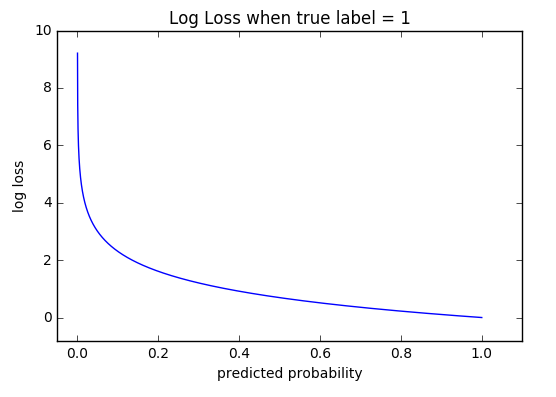
\includegraphics[width=\linewidth]{cross_entropy.png}
        
        \paragraph{NegativeLogLikelihoodLoss} \tab $ \operatorname { NLLLoss } ({logs }, \text {true label} ) = - logs[\text { true label }]$, where for logs the following should be used to make it equal to the \textit{Cross-entropy loss}: $logs=log(softmax(x))$

		\section{Adverserial Examples}
			
			\subsection*{Targeted FGSM (Fast Gradient Sign Method)}
			
			     Intuition: Goal is to perturbe the image such that the NN missclassifies the image to target label $\boldsymbol t$. Therefore \textbf{reduce} the loss of the \textbf{target} label.
			     
			     \begin{tabbing}
			     0. Target label $\boldsymbol t$, true label $\boldsymbol s$, generally $t \neq s$ \\
				 1. Compute perturbation: \hspace{2mm} \= $\eta = \epsilon \cdot \operatorname { sign } \left( \nabla _ { x } \operatorname { loss } _ { t } ( x ) \right)$ \\
				
				\> $\nabla _ { x } \operatorname { loss } _ { t } = \left( \frac { \partial \operatorname { loss } _ { t } } { \partial x _ { 1 } } , \ldots , \frac { \partial \operatorname { loss } _ { t } } { \partial x _ { n } } \right)$ \\
				\> $ \text{,where } \operatorname { loss } _ { t } \text{is the entry of the}$  \\ 
				\> $ \text{cross entropy loss vector for}$  \\
				\> $ \text{the target label}$ and $x$ is the \\
				\> image vector.\\
				
				2. Perturb the input: \> $x ^ { \prime } = x - \eta$ \\
				3. Check if: \> $f \left( x ^ { \prime } \right)= t$, where $f \left( x \right) $ \\
				\> is classification result of the \\
				\> NN for $x$.
			\end{tabbing}
			
			\subsection*{{\color{red}Un}targeted FGSM (Fast Gradient Sign Method)}
			\begin{tabbing}
			     0. True label ${\color{red} s}$ \\
				 1. Compute perturbation: \hspace{2mm} \= $\eta = \epsilon \cdot \operatorname { sign } \left( \nabla _ { x } \operatorname { loss } _ { \mathbin{\textcolor{red}s}} ( x ) \right)$ \\
				
				\> $\nabla _ { x } \operatorname { loss } _ { \mathbin{\textcolor{red}s}} = \left( \frac { \partial \operatorname { loss } _ { {\color{red}s}} } { \partial x _ { 1 } } , \ldots , \frac { \partial \operatorname { loss } _ { {\color{red}s}} } { \partial x _ { n } } \right)$ \\

				
				2. Perturb the input: \> $x ^ { \prime } = x \mathbin{\textcolor{red}+} \eta$ \\
				3. Check if: \> $f \left( x ^ { \prime } \right)  \mathbin{\textcolor{red}\neq s}$
			\end{tabbing}
			
			\subsection*{PGD (Projected Gradient Descent)}
			Take $\boldsymbol{k}$ steps of \textbf{FGSM} each of size $\epsilon$. After each step project onto $S ( x )$. By projecting, we mean that we find the closest point inside the $ S ( x )$  ball (e.g. $L_{\infty}$ ball). Here, closest is defined according to some norm (e.g. $L_{\infty}$). In the region of $S(X)$ we want all point to be classified with the \textbf{same} label.
			\\
			$S ( x ) = \left\{ x ^ { \prime } | \left\| x - x ^ { \prime } \right\| _ { \infty } < \epsilon \right\}$

			Note that the $S ( x ) $ ball is of size $\boldsymbol \epsilon $ which is different than the $ \boldsymbol{ \epsilon _ {\color{green} step }  }$ of the {\color{green}FGSM step} and normally it holds that $\epsilon _ {\color{green} step } < \epsilon $.
			
			Projecting on the $L_{\infty}$ ball is the same as clamping the values: $x ^ { \prime }_{projected} = clamp(x ^ { \prime }, min=x-\epsilon, max= x+\epsilon)$ \\
			Note that the resulting $x ^ { \prime }_{projected}$ can be inside the $L_{\infty}$ ball.
			\\
		\textbf{Minimization Problem for Defense:}
			
			$\left. \begin{array} { l l } { \text { find } } & { \theta } \\ 
			{ \text { minimize } } & {{\color{green} \rho ( \theta ) }} \\ 
			{\text { where } } & { \rho ( \theta ) = \mathbf { E } _ { ( x , y ) \sim D } \left[ \mathbin{\textcolor{red} \max _ { x ^ { \prime } \in S ( x ) } L \left( \theta , x ^ { \prime } , y \right)} \right]} \\
			{ \text { in practice } } & { \rho ( \theta ) = \frac { 1 } { \left| D _ { a } \right| } \sum _ { ( x , y ) \in D a } L ( \theta , x , y ) } \end{array} \right.$, \\
			where  $D _ { a }$ is dataset of adverserial examples
			
			For which ${{\color{green} \rho ( \theta ) }}$ is the empirical risk (Loss) and the {\color{green} outer } optimization ({\color{green}min}) problem (Defense): \textit{Find $\theta$ that minimizes the high loss $\rightarrow$ train robust classifier} (with normal SGD methode $\theta' = \theta - \epsilon_{\text{learning rate}} \cdot \nabla _ { \theta } \rho ( \theta )$.)
			
			Further, $\mathbin{\textcolor{red} \max _ { x ^ { \prime } \in S ( x ) } L \left( \theta , x ^ { \prime } , y \right)}$ the {\color{red} inner} optimization ({\color{red}max}) problem (Attack): \textit{Find adverserial $x\prime$ achieves high loss  $\rightarrow$ adverserial attack.}
		
            \subsection*{Optimization Problem}
            Objective is to have a \textbf{small} perturbation $\eta$, such that the image is missclassified. Large perturbation is not wanted:
            $\begin{array} { l l } { \text { find } } & { \eta } \\ { \text { minimize } } & { \| \boldsymbol { \eta } \| _ { p } } \\ { \text { such that } } & { f ( x + \eta ) = t } \\ { } & { x + \boldsymbol { \eta } \in [ 0,1 ] ^ { n } } \end{array}$\\
            In general this is a hard problem to optimize with gradient descent. Therefore ease the constrains.
            \begin{enumerate}[leftmargin=*]
            \item
            Use \textbf{objective function}:\\
            $o b j ( x + \eta ) \leq 0\quad \Rightarrow \quad f ( x + \eta ) = t$\\
            A correct objective function is a function that has
            $o b j ( x') \leq 0 \iff p(t) \geq 0.5$\\
            \\
            Sound objective functions for \textbf{2-class} NN:\\
            $o b j \left( x ^ { \prime } \right) = \operatorname { loss } _ { t } \left( x ^ { \prime } \right) - 1$\\
            $o b j \left( x ^ { \prime } \right) = \max \left( 0,0.5 - \text{softmax}\left(x ^ { \prime }\right) _ { t } \right)$\\
            For \textbf{$\mathbf{k}$-class} NN this is:\\
            $\mathrm { obj } _ {\boldsymbol{k} }(\boldsymbol{x}^ \prime)  = - \log _ {\mathbf{k}} \left( \text{softmax}\left(x ^ { \prime }\right) _ { t } \right) - 1 = C \cdot \operatorname { loss } _ { t } \left( \boldsymbol { x } ^ { \prime } \right) - 1$,\\
            where $C = \frac { 1 } { \log _ { 2 } ( \boldsymbol{k} ) }$ for cross-entropy loss with $\log _ { 2 }$.
            
            \item
            Replace norm with \textbf{proxy function} because the gradient of e.g. the inf norm is zero for most values except the maximum value.\\
            Replace $\| \boldsymbol { \eta } \| _ { \infty }$ with $\sum _ { i } \max \left( 0 , \left( \boldsymbol { \eta } _ { i } - \tau \right) \right)$\\
            If all entries are less then $\tau$ then the entire expression is zero.
            Note: When $\tau$ is large, the gradient is similar to the gradient of $\| \eta \| _ { \infty }$.
            Start with large $\tau$ and lower after each iteration.
            
            \item
            Clamp perturbed image back to box domain after optimization.
            \end{enumerate}
            Then the optimization becomes:\\
            $\begin{array} { l l } { \text { find } } & { \eta } \\ { \text { minimize } } & { \| \boldsymbol { \eta } \| _ { p } + c \cdot o b j ( x + \boldsymbol { \eta } ) } \\ { \text { such that } } & { x + \eta \in [ 0,1 ] ^ { n } } \end{array}$
            
            \subsection*{Diffing Networks}
            Given two NN trained to learn same function. Perturb Input $x$ such that $class(f_1(x')) \neq class(f_2(x'))$ 
            
            Use the following objective function, where $f_i(x')_t$ is the softmax output of of NN $i$ w.r.t. 
            
            \textbf{while} $\operatorname { class } \left( f _ { 1 } ( x ) \right) = \operatorname { class } \left( f _ { 2 } ( x ) \right) :$\\
            $\null \quad o b j ( x ) = f _ { 1 } ( x ) _ { t } - f _ { 2 } ( x ) _ { t } \rightarrow$ Use as Loss\\
            $\null \quad x = x \mathbin{\textcolor{red}{ + }} \epsilon \cdot \frac { \partial o b j ( x ) } { \partial x } \quad \rightarrow $ {\color{red} Maximize } Loss\\
            \textbf{return} $x$
        
        \newpage
		\section{Logic}
		    Goal: Want to query NN such that some logical constrains are satisfied.\\
		    Problem: Formulating this as a constrained problem is hard to solve and times out for large NN.\\
		    Solution: Translate logical constrain into loss.
			\subsection*{Translations}
			$\forall \mathrm { x } ,$ if $\mathrm { T } ( \phi ) ( \mathrm { x } ) = 0 \Rightarrow \phi(x)$ satisfied, \\where $\phi(x)$ is logical formula
			
			Use the following constrains to generate loss function.
            \begin{center}
            \begin{tabular}{@{}lll@{}}
            Logical Term                                       & Translation                                                                                                                     & Logic Negation ($\neg$)                                                   \\ \midrule
            $t _ { 1 } = t _ { 2 }$                            & $\left| t _ { 1 } - t _ { 2 } \right|$                                                                                          & $\mathrm { t } _ { 1 } < \mathrm { t } _ { 2 } \vee \mathrm { t } _ { 2 } < \mathrm { t } _ { 1 }$ \\
            $\mathrm { t } _ { 1 } \leq \mathrm { t } _ { 2 }$ & $\max \left( 0 , t _ { 1 } - t _ { 2 } \right)$                                                                                 & $\mathrm { t } _ { 1 } > \mathrm { t } _ { 2 }$                                                    \\
            $t _ { 1 } < t _ { 2 }$                            & $\mathrm { T } \left( \mathrm { t } _ { 1 } + \epsilon \leq \mathrm { t } _ { 2 } \right)$                                      & $t _ { 1 } \geq t _ { 2 }$                                                                         \\
            $t _ { 1 } \neq t _ { 2 }$                         & $\mathrm { T } \left( \mathrm { t } _ { 1 } < \mathrm { t } _ { 2 } \vee \mathrm { t } _ { 2 } < \mathrm { t } _ { 1 } \right)$ & $t _ { 1 } = t _ { 2 }$                                                                            \\
            $\varphi \vee \psi$                                & $T ( \varphi ) \cdot T ( \psi )$                                                                                                & $\neg \varphi \wedge \neg \psi$                                                                    \\
            $\varphi \wedge \psi$                              & $T ( \varphi ) + T ( \psi )$                                                                                                    & $\neg \varphi \vee  \neg \psi$                                                                     \\ \bottomrule
            \end{tabular}
            \end{center}
            Problem: When dealing with \textbf{real} values in logical domain and \textbf{floats} in loss domain one has to assign $\epsilon$ to smallest machine value. Thereafter Translation is only valid in one direction ($\mathrm { T } ( \phi ) ( \mathrm { x } ) = 0 \Rightarrow \phi(x)$ satisfied). It no longer holds that when $\phi(x)$ satisfied, that the loss is 0.\\
            E.g. $t_1 < t_2 \Rightarrow T(\phi) =\max (0, t_1 + \epsilon - t_2) $\\
            Use, $t_1 = t_2 - \frac{\epsilon}{2}$.
            It holds that $t_1 < t_2$ but Translation is not satisfied since $T(\phi) = \max (0, t_2 - \frac{\epsilon}{2}- t_2 ) = \frac{\epsilon}{2} \neq 0$\\
            Therefore, $\mathrm { T } ( \phi ) ( \mathrm { x } ) = 0 \Rightarrow \phi(x)$ satisfied, \\but $ \phi(x) \text{satisfied} \centernot{\xRightarrow{}} \mathrm { T } ( \phi ) ( \mathrm { x } ) = 0$
            \subsection*{Example}
                Goal: Find an image i which
                        gets classified to 9
                        where the image i is
                        within some distance
                        of the image deer.
             \begin{enumerate}[leftmargin=*]
             \setcounter{enumi}{-1} 
            \item Logical Formula:\\
            $\phi(i) = \bigwedge _ { \mathrm { j } = 1 , j \neq 9 } ^ { \mathrm { k } } \mathrm { NN } ( \mathrm { i } ) [ \mathrm { j } ] < \mathrm { NN } ( \mathrm { i } ) [ 9 ] \wedge \| \mathrm { i } - \operatorname { deer } \| _ { \infty } < 25 \\ \null \hspace{5.8cm} \wedge \| \mathrm { i } - \operatorname { deer } \| _ { \infty } > 5$
            \item Translation into loss:\\
            $\begin{aligned}
            T (\phi)  & =
            {\sum}_ { \mathrm { j } = 1 , j \neq 9 } ^ { \mathrm { k }} \max ( 0 , \mathrm { NN } ( \mathrm { i } ) [ j ] + \epsilon - \mathrm { NN } ( \mathrm { i } ) [ 9 ] \\
            & \quad + { \max ( 0 ,  \| \mathrm { i } - \operatorname { deer } \| _ { \infty } + \epsilon - 25 )} \\ 
            & \quad + { \max ( 0 , } 5 + \epsilon - \| \mathrm { i } - \operatorname { deer } \| _ { \infty })\\
            \end{aligned}$
            \item Train Network with SGD
            
            \end{enumerate}
		    \subsection*{Train NN with Logic}
		    \begin{enumerate}[leftmargin=*]
		    \setcounter{enumi}{-1}
		    \item
		    Goal: Want to enforce property $\phi$.
		    Find weights for NN, such that expected value of the property increases:\\
            $\begin{array} { l l } { \text { find } } & { \theta } \\ { \text { maximize } } & { \rho ( \theta ) } \\ { \text { where } } & { \rho ( \theta ) = \mathbf { E } _ { s - D } [ \forall \mathbf { z } \cdot \phi ( \mathbf { z } , s , \theta ) ] } \end{array}$
            \item Translate into loss:\\
            $\begin{array} {l l l l } 
            { \text { find } } & { \theta } \\ { \text { minimize }}  & { \rho ( \theta )} \\
            { \text { where } } & {\rho ( \theta ) = \mathbf { E } _ { s \sim D } \left[ \mathrm { T } ( \phi ) \left( z _ { \text { worst }} , s , \theta \right) \right]} \\
            {\text{and}} & {z _ {\text { worst }} = \arg \min _ { Z } ( \mathrm { T } ( \neg \phi ) ( z , s , \theta ) )}
            \end{array}$\\
            Inner minimization: Find worst violation of property.\\
            Outer minimization: Find weight such that worst violation is minimized.\\
            Intuitively, we are trying to get the
            worst possible violation of the formula and then to find a
            network that minimizes its effect.\\
            \item Solve inner minimization by splitting loss:\\
            e.g.
            $\begin{aligned}[t]
            \operatorname { loss } ( z , x , \theta ) &= \max \left( 0 , \| x - z \| _ { \infty } - \epsilon \right) \\
            & + \max \left( 0 , N N _ { \theta } ( z ) [ 3 ] - \delta \right)
            \end{aligned}$\\
            
            $\rightarrow$ split loss!
            \begin{enumerate}[label*=\arabic*.]
                \item Solve with PGD: \\
                $\min _ { z } \operatorname { loss } ( z , x , \theta ) = \max \left( 0 , N N _ { \theta } ( z ) [ 3 ] - \delta \right)$
                \item Project $z$ back onto the $L _ { \infty } ( x , \epsilon )$ ball
            \end{enumerate}
            
            
            
            \end{enumerate}
            
		\section{Certifay AI - Abstract Domains}
		    \textbf{Sound:} Correct Approximation of NN.\\
		    \textbf{Precise:} Approximation is superset of NN, but should not approximate too much, otherwise can not verify NN.\\
		    \textbf{Efficient:} Efficient to compute
			\subsection*{Interval Domain}
			Input $x$ is in the form of $x = [a,b]$. \\
			
			\textbf{Operation Rules}\\
			Addition: $x_1+x_2 = [x_1[0] + x_2[0], x_1[1] + x_2[1]]$\\
			Substract.: $[x_1, x_2] - [y_1, y_2] = [x_1-y_2, x_2-y_1]$\\
			Addition Scalar: $x_1+a = [x_1[0] + a, x_1[1] +a]$\\
			Multipl.: $\begin{aligned}[t]  [x_1, x_2] \cdot [y_1, y_2] & = [\min(x_1 y_1,x_1 y_2,x_2 y_1,x_2 y_2), \\ 
			& \qquad \max(x_1 y_1,x_1 y_2,x_2 y_1,x_2 y_2)]\end{aligned}$\\
			Multipl Scalar: $x_1 \cdot a = [l, u], \\ 
			\text{with } l= min(x[0]\cdot a, x[1] \cdot a), u = max(x[0] \cdot a, x[1]\cdot a)$\\
			Funct.: $\begin{aligned}[t]
			f([y_{1},y_{2}]) & = [ \min \left\{f(y_{1}),f(y_{2})\right\},\\
			& \qquad \max \left\{f(y_{1}),f(y_{2})\right\} ] \end{aligned}$\\
			Lower Equal: $\begin{aligned}[t] \leq \left( \left[ l _ { 1 } , u _ { 1 } \right] , \left[ l _ { 2 } , u _ { 2 } \right] \right) & = ( \left[ l _ { 1 } , u _ { 1 } \right] \sqcap _ { i } \left[ - \infty , u _ { 2 } \right]  \\
			& \quad , \left[ l _ { 1 } , \infty \right] \sqcap _ { i } \left[ l _ { 2 } , u _ { 2 } \right])\end{aligned}$
			\subsection*{Zonotope Abstrac Domain}
			$\hat { m } = a _ { 0 } ^ { m } + \sum _ { i = 1 } ^ { k } a _ { i } ^ { m } \epsilon _ { i }$\\
			$\epsilon _ { i } :$ noise terms ranging $[ - 1,1 ]$ shared between abstract neurons\\
			$a _ { i } ^ { n } :$ real number that controls magnitude of noise\\
			Centered around $a _ { 0 } ^ { m }$\\
			\textbf{Operation Rules}\\
			\textbf{Multiplication with scalar}\\
			$\left( a _ { 0 } ^ { n } + \sum _ { i = 1 } ^ { k } a _ { i } ^ { n } \epsilon _ { i } \right) \cdot C = \left( C \cdot a _ { 0 } ^ { n } + \sum _ { i = 1 } ^ { k } C \cdot a _ { i } ^ { n } \epsilon _ { i } \right) \text{,} C \in \mathbb{R} $\\
			\textbf{Multiplication of two variable}\\
			\begin{multline*}
    			\left( a _ { 0 } ^ { n } + \sum _ { i = 1 } ^ { k } a _ { i } ^ { n } \epsilon _ { i } \right) \cdot \left( a _ { 0 } ^ { m } + \sum _ { i = 1 } ^ { k } a _ { i } ^ { m } \epsilon _ { i } \right) = \left( a _ { 0 } ^ { n } \cdot a _ { 0 } ^ { m } \right) + \\
    			\sum _ { i = 1 } ^ { k } \left( a _ { i } ^ { n } \cdot a _ { 0 } ^ { m } + a _ { i } ^ { m } \cdot a _ { 0 } ^ { n } \right) \cdot \epsilon _ { i } + \sum _ { i = 1 } ^ { k } \sum _ { j = 1 } ^ { k } a _ { i } ^ { m } \cdot a _ { j } ^ { n } * \epsilon_i \cdot \epsilon_j
			\end{multline*}
			where $\epsilon _ { i } \cdot \epsilon _ { j }$ becomes new variable $\epsilon _ { i, j }$ and \\
			$\begin{array} { l l } { \epsilon _ { i , j } \in [ - 1,1 ] \text { if } i \neq j } \\ 
			{\epsilon _ { i , j } \in [ 0,1 ] \text { if } i = j } \end{array}$\\

			\textbf{Summation}\\
			$\begin{aligned}
			\left( a _ { 0 } ^ { n } + \sum _ { i = 1 } ^ { k } a _ { i } ^ { n } \epsilon _ { i } \right) + \left( a _ { 0 } ^ { m } + \sum _ { i = 1 } ^ { k } a _ { i } ^ { m } \epsilon _ { i } \right) & = \left( a _ { 0 } ^ { n } + a _ { 0 } ^ { m } \right) \\
			& + \sum _ { i = 1 } ^ { k } \left( a _ { i } ^ { n } + a _ { i } ^ { m } \right) \cdot \epsilon _ { i }
			\end{aligned}$\\
			
			\textbf{Join}\\
			Operation is not closed. Example of the Operation:\\
			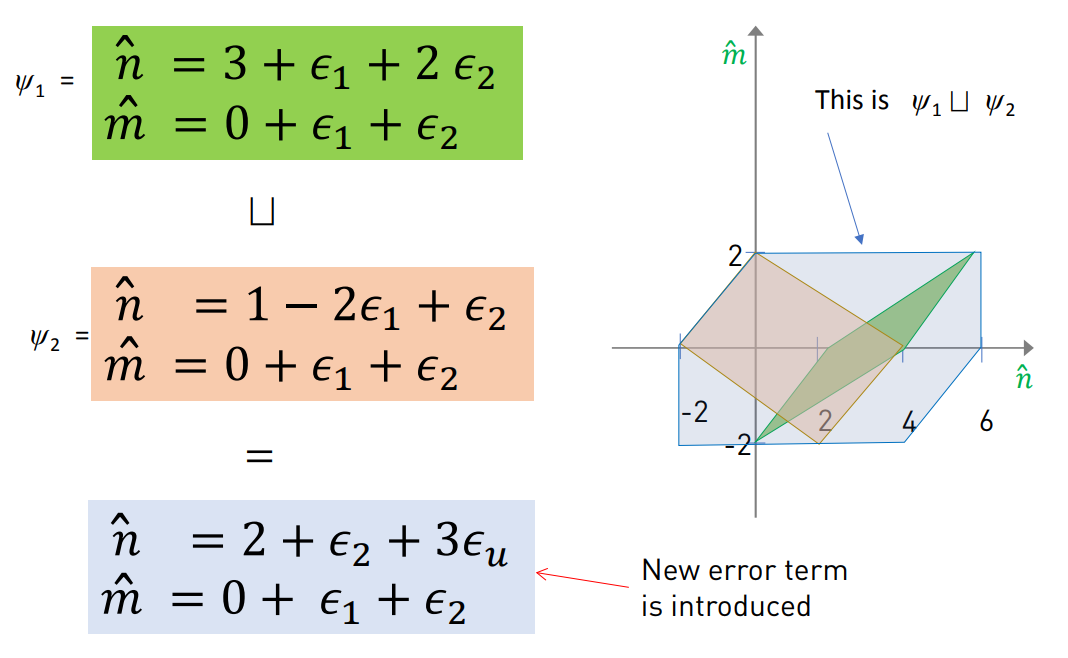
\includegraphics[width=\linewidth]{join_polytope.png}\\
			\textbf{ReLU}\\
			$\begin{array} { l l }
			{ f _ { R e L U } ^ { \# } = \operatorname { Re } L U _ { 2 } ^ { \# } ( b ) \circ \operatorname { Re } L U _ { 1 } ^ { \# } ( a ) \text { (Affine) } } \\
			\operatorname {ReLU} _ { i } ^ { \# } \left( x _ { i } \right) ( \psi ) =
			\mathbin{\textcolor{red} {\psi_ { \left\{ x _ { i } \geq 0 \right\}}}}
			\sqcup  \mathbin{\textcolor{green}{\psi _ {\left\{ x _ { i } < 0 \right\}} \quad \text{,} }}
			\end{array} $ \\
			where
			$  \mathbin{\textcolor{red} {\psi_ { \left\{ x _ { i } \geq 0 \right\}}}} = 
			\left( \psi \sqcap \left\{ x _ { i } \geq 0 \right\} \right)$ , for which $\sqcap$ is not defined.\\
			and
			$ \mathbin{\textcolor{green}{\psi _ {\left\{ x_{ i } < 0 \right\}} }} = \left\{ \begin{array}{ c l } { \left[ \left[ x _ { i } = 0 \right] \right] ( \psi ) } & { \text { if } \left( \psi \cap \left\{ x _ { i } < 0 \right\} \right) \neq \perp } \\ { \perp } & { \text { otherwise } } \end{array} \right.$\\
			
			\newpage
			\textbf{Box}\\
			$\begin{aligned}
			z_{box} = & \Bigg[ 
			\left( a _ { 0 } ^ { n } + \sum _ { i = 1 } ^ { k } a _ { i } ^ { n } \cdot {\operatorname{sign}}(a _ { i } ^ { n })\cdot (-1)  \right), \\
			& \left( a _ { 0 } ^ { n } + \sum _ { i = 1 } ^ { k } a _ { i } ^ { n } \cdot {\operatorname{sign}} (a _ { i } ^ { n }) \right) \Bigg]
			\end{aligned}$
			
		\subsection{Train provable robust NN}
		$\begin{array} { l l }
		{ \text { find } } & { \theta } \\ { \text { minimize } } & { \rho ( \theta ) } \\ { \text { where } } & { \rho ( \theta ) = \mathbf { E } _ { ( x y ) \sim D } \left[ \max _ { z \in \gamma \left( N N ^ { * } ( \alpha ( S ( x ) ) ) \right. } L ( \theta , z , y ) \right] }
		\end{array}$\\
		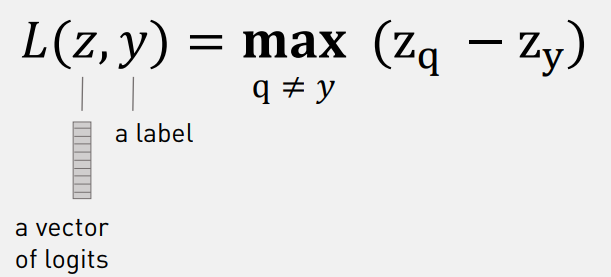
\includegraphics[width=6cm]{Loss_abstract.png}\\
		Set of $z$ can be large. Instead of enumerate the set first transform it. For each $z_q$ use the following: \\
		$d_q = z_q - z_y$ and then $u_q = \max \left( \operatorname { box } \left( d _ { q } \right) \right)$
		where $u_q$ is the upper bound of the polytope $d_q$ transformed into the box domain. Therefore,
		
		$L ( z , y ) = \max _ { q \neq y } \left( z _ { q } - z _ { y } \right) = \max _ { q} (u_q )$
		
		\section{Visualize CNN}
		    \textbf{Early} layers are Gabor-filter-like filters for edges.\\
		    \textbf{Later} layers have more complex, abstract patterns.\\
		    \subsection*{Feature Visualization} Template that the NN is looking for.\\
		    \textbf{First layers as Images}:\\
		    Interpret weights of layers as images. Only works for layers with up to 3 channels.\\
		    \textbf{Visualization by Optimization:}
		    \begin{enumerate}[leftmargin=*]
                \item Initialize input image with noise.
    		    \item Maximize response of a channel of a certain later. For that define score, i.e.
    		    score $( x ) = \operatorname { mean } \left( \operatorname { layer } _ { n } [ : , : ; , 3 ] \right)$
    		    \item Use SGD to update input image and add regularization term so that image is constraint to look like an image: $x \leftarrow x + \eta \nabla _ { x } \operatorname { score } ( x ) + \sum _ { t } \lambda _ { t } R _ { t } ( x )$\\
    		    Regularization: E.g. penalyze high frequencies
		    \end{enumerate}
		    \textbf{Early} layers produce strong line patterns.\\
		    While \textbf{later} layers show higher level concepts.\\
		    
		    \vspace{1cm}
		    \subsection*{Attribution} Location/pixels that are important for NN decision.\\
		    \textbf{Grad-CAM}\\
		    Highlight region of image that activates layer for some label $s$.\\
	        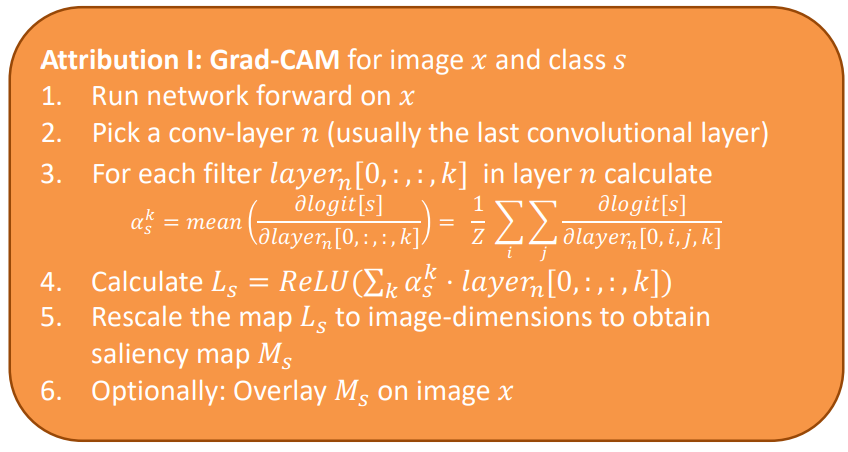
\includegraphics[width=\linewidth]{attribution.png}\\
	        Where, 
	        $L _ { S } = \operatorname {ReLU} {\bigg (} \sum _ { k } \underbrace { \alpha _ { S } ^ { k }}_{\substack{\text{Importance}\\ \text{of class s}}} \cdot \underbrace {\operatorname { layer } _ { n } [ 0 , : ; ; k ] ) } _ { \text { Spatial Activations } } {\bigg )}$\\
	        \textbf{Meaningful Perturbations}\\
	        Learn which part of image can be perturbed such that the NN will predict wrong label.\\
			\subsection*{Non Negative Matrix Factorization (NMF)}	
			$\mathbf {W} \mathbf {H} = \mathbf {V}  $\\
		    $\mathbf {W}\in \mathbb{R}^{r \times k}, \quad \mathbf {H}\in \mathbb{R}^{k \times c}, \quad \mathbf {V} \in \mathbb{R}^{r \times c} $\\
		    Columns in $\mathbf {H} $ correspond to patterns in $\mathbf {V}$. Whereas rows in $\mathbf {W} $ contain weights for those patterns.\\
	        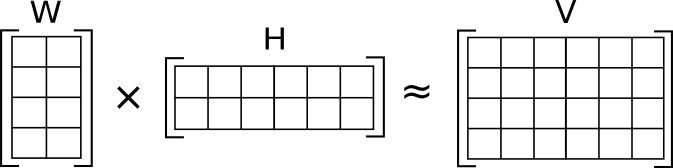
\includegraphics[width=\linewidth]{NMF.png}\\
	        Use NMF on post-ReLU activation of last convolutional layer. Thereafter use feature visualization with help of optimization to visualize the patterns. Can also be used for attribution by thresholding the prototypes and combining them.
        \section{Probabilistic Programming}
        $P(A_{i}\mid B)={\frac {P(B\mid A_{i})\,P(A_{i})}{\sum \limits _{j}P(B\mid A_{j})\,P(A_{j})}}\cdot $\\
        \textbf{Distributions}
        \texttt{x := Distribution}\\
        \texttt{
        uniform(a,b)\\
        uniformInt(a,b)\\
        gauss(mean,variance)\\
        bernoulli(p)\\
        poisson(mean)\\
        }
        \textbf{Obvervations}
        \texttt{observe (x >= 0.5)}
        \subsection*{Examples}
        Run a \textit{psi} program with \texttt{psi
dice.psi --expectation} The \texttt{--expectation} flag is used to get the probability. Without the flag the exact distribution (PDF) is returned.
        \begin{Verbatim}[numbers=left,xleftmargin=5mm, fontsize=\small]
def main(){ // didItRain
cloudy := flip(0.5);
rain := 0; sprinkler := 0;

if (cloudy){
    rain = flip(0.8);
    sprinkler = flip(0.1);
}else{
    rain = flip(0.2);
    sprinkler = flip(0.5);
}

wetGrass := rain || sprinkler;

observe(wetGrass);
return rain==1; // Probability that it rains,
                // given grass is wet.
} 
        \end{Verbatim}
    	\begin{Verbatim}[numbers=left,xleftmargin=5mm, fontsize=\small]
def main(){ // Dice
n := 40;
sum := 0;
for i in [0..n){
    dice := uniformInt(1,6);
    sum += dice;
}
average := sum / n;
return average > 4; // Prob. that average of 40...
                    // dice throws is above 4.
}
	\end{Verbatim}
	    	\begin{Verbatim}[numbers=left,xleftmargin=5mm, fontsize=\small]
def main(){ // Dice 2
n := 20;
sum := 0;
n_6 := 0;
for i in [0..n){
    roll := uniformInt(1,6);
    sum += roll;
    if roll == 6{
        n_6 += 1;
    }
}
average := sum / n;
observe(n_6 >= 10);
eturn average > 4; // Prob. that average of 20...
                // dice throws is above 4, given
                // at least 10 rolls are a 6.
}
            \end{Verbatim}
            \newpage
	    	\begin{Verbatim}[numbers=left,xleftmargin=5mm, fontsize=\small]
def main(){ \\ Program with expectation of Pi.
    x := uniform(0,1);
    y := uniform(0,1);
    within_radius := x*x+y*y <= 1;
    return 4*within_radius; \\Prob. that point ...
                            \\is within radius.
}
        \end{Verbatim}
    \subsection*{Differential Privacy}
    \textbf{Epsilon - Differential Privacy}\\
	$\frac { \operatorname { Pr } [ F ( x ) \in \Phi ] } { \operatorname { Pr } \left[ F \left( x ^ { \prime } \right) \in \Phi \right] } \leq \exp ( \varepsilon )$\\
	, where $F ( x )$ is the output of the database query including randomization,  $x ^ { \prime }$ is a database that differs on a single element w.r.t. to $x$ and $\Phi$ is the secret.

\section{Programming by Examples (PBE)}
A new frontier in AI where one learns an
interpretable program from user-provided examples. \\
Requires very few input-output examples.
Assumes the given examples are representatives.
\subsection*{PBE problem definition}
\textbf{Given:} A domain specific Language (DSL) \& set of input-output examples.\\
\textbf{Goal:} Learn a function over the DSL which is consistent with the provided examples.\\


	\end{multicols*}



\end{document}
